\documentclass{article}
\usepackage{tikz}
\usepackage{amssymb}
\pagestyle{empty}
\begin{document}
% GEOMIRA export: TikZ. One unit is 23.606798bp (31.47573 px on screen).
% Needs \usepackage{tikz} and \usepackage{amssymb}.
% Warning: O* is undefined in this figure (apply: the point is the center of inversion: its image is at infinity): not drawn
% Warning: tri* is undefined in this figure (apply: an inversion maps the sides of a polygon to arcs, so it has no image): not drawn
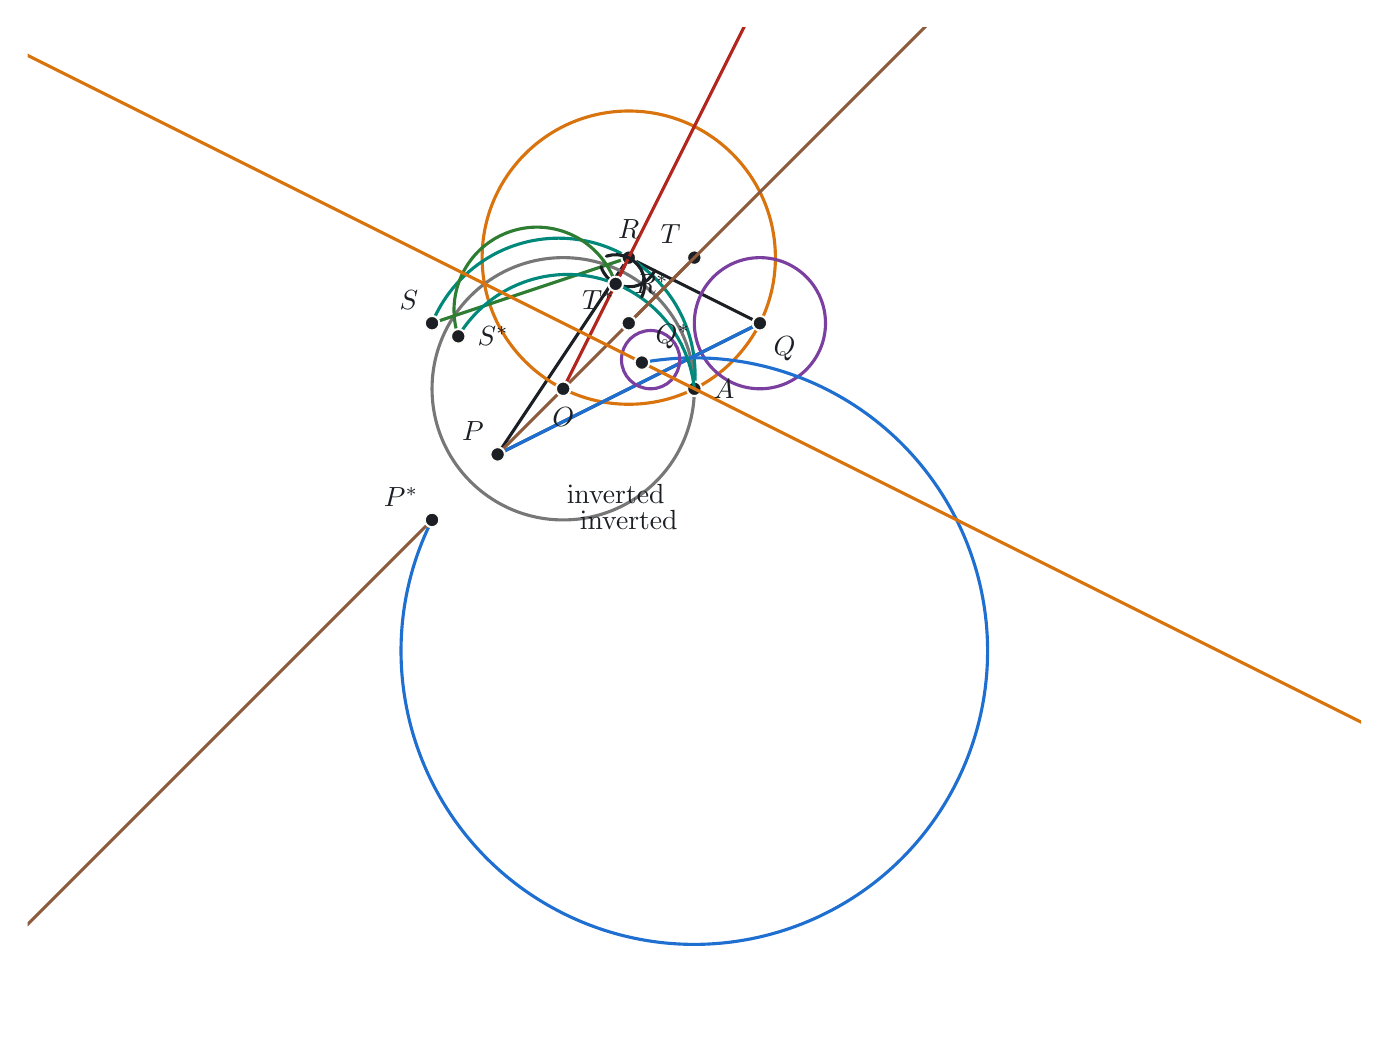
\begin{tikzpicture}[x=23.606798bp, y=23.606798bp, line cap=round, line join=round]
\definecolor{gmc0}{HTML}{1B1F24}
\definecolor{gmc1}{HTML}{777777}
\definecolor{gmc2}{HTML}{D9730D}
\definecolor{gmc3}{HTML}{7B3FA0}
\definecolor{gmc4}{HTML}{00897B}
\definecolor{gmc5}{HTML}{1F6FD1}
\definecolor{gmc6}{HTML}{8D5A3B}
\definecolor{gmc7}{HTML}{B3261E}
\definecolor{gmc8}{HTML}{2E7D32}
\definecolor{gmc9}{HTML}{FBFBF8}
\clip (-8.1666,-9.743) rectangle (12.1666,5.5069);
% tri
\draw[gmc0, line width=1.125bp] (-1,-1) -- (3,1);
\draw[gmc0, line width=1.125bp] (3,1) -- (1,2);
\draw[gmc0, line width=1.125bp] (1,2) -- (-1,-1);
% w
\draw[gmc1, line width=1.125bp] (2,0) arc[start angle=0, end angle=360, radius=2];
% k
\draw[gmc2, line width=1.125bp] (3.2361,2) arc[start angle=0, end angle=360, radius=2.23607];
% c
\draw[gmc3, line width=1.125bp] (4,1) arc[start angle=0, end angle=360, radius=1];
% a
\draw[gmc4, line width=1.125bp] (2.0111,0.2143) arc[start angle=0, end angle=157.8337, radius=2.08248];
\draw[gmc4, line width=1.125bp] (2,0) arc[start angle=354.0939, end angle=360, radius=2.08248];
% pq
\draw[gmc5, line width=1.125bp] (-1,-1) -- (3,1);
% pt
\draw[gmc6, line width=1.125bp] (-1,-1) -- (2,2);
% oq
\draw[gmc7, line width=1.125bp] (0,0) -- (1,2);
% sr
\draw[gmc8, line width=1.125bp] (-2,1) -- (1,2);
% m
\draw[gmc0, line width=1.125bp] (0.578,1.8593) arc[start angle=-161.5651, end angle=-26.5651, radius=0.44479];
% O
\filldraw[fill=gmc0, draw=gmc9, line width=0.75bp] (0,0) circle[radius=2.625bp];
% A
\filldraw[fill=gmc0, draw=gmc9, line width=0.75bp] (2,0) circle[radius=2.625bp];
% P
\filldraw[fill=gmc0, draw=gmc9, line width=0.75bp] (-1,-1) circle[radius=2.625bp];
% Q
\filldraw[fill=gmc0, draw=gmc9, line width=0.75bp] (3,1) circle[radius=2.625bp];
% R
\filldraw[fill=gmc0, draw=gmc9, line width=0.75bp] (1,2) circle[radius=2.625bp];
% S
\filldraw[fill=gmc0, draw=gmc9, line width=0.75bp] (-2,1) circle[radius=2.625bp];
% T
\filldraw[fill=gmc0, draw=gmc9, line width=0.75bp] (2,2) circle[radius=2.625bp];
% t
% pq*
\draw[gmc5, line width=1.125bp] (6.4721,-4) arc[start angle=0, end angle=100.3048, radius=4.47214];
\draw[gmc5, line width=1.125bp] (-2,-2) arc[start angle=153.4349, end angle=360, radius=4.47214];
% sr*
\draw[gmc8, line width=1.125bp] (0.8,1.6) arc[start angle=18.4349, end angle=198.4349, radius=1.26491];
% c*
\draw[gmc3, line width=1.125bp] (1.7778,0.4444) arc[start angle=0, end angle=360, radius=0.44444];
% a*
\draw[gmc4, line width=1.125bp] (2,0) arc[start angle=5.9061, end angle=149.0362, radius=1.94365];
% pt*
\draw[gmc6, line width=1.125bp] (-10.327,-10.327) -- (-2,-2);
\draw[gmc6, line width=1.125bp] (1,1) -- (7.6673,7.6673);
% oq*
\draw[gmc7, line width=1.125bp] (0.8,1.6) -- (3.8336,7.6673);
% k*
\draw[gmc2, line width=1.125bp] (-10.327,6.1635) -- (14.327,-6.1635);
% m*
\draw[gmc0, line width=1.125bp] (1.1978,1.4011) arc[start angle=-26.5651, end angle=108.4349, radius=0.44479];
% P*
\filldraw[fill=gmc0, draw=gmc9, line width=0.75bp] (-2,-2) circle[radius=2.625bp];
% Q*
\filldraw[fill=gmc0, draw=gmc9, line width=0.75bp] (1.2,0.4) circle[radius=2.625bp];
% R*
\filldraw[fill=gmc0, draw=gmc9, line width=0.75bp] (0.8,1.6) circle[radius=2.625bp];
% S*
\filldraw[fill=gmc0, draw=gmc9, line width=0.75bp] (-1.6,0.8) circle[radius=2.625bp];
% T*
\filldraw[fill=gmc0, draw=gmc9, line width=0.75bp] (1,1) circle[radius=2.625bp];
% t*
\node[anchor=north, inner sep=0pt, text=gmc0] at (0,-0.2859) {$O$}; % label of O
\node[anchor=west, inner sep=0pt, text=gmc0] at (2.2859,0) {$A$}; % label of A
\node[anchor=south east, inner sep=0pt, text=gmc0] at (-1.2022,-0.7978) {$P$}; % label of P
\node[anchor=north west, inner sep=0pt, text=gmc0] at (3.2022,0.7978) {$Q$}; % label of Q
\node[anchor=south, inner sep=0pt, text=gmc0] at (1,2.2859) {$R$}; % label of R
\node[anchor=south east, inner sep=0pt, text=gmc0] at (-2.2022,1.2022) {$S$}; % label of S
\node[anchor=south east, inner sep=0pt, text=gmc0] at (1.7978,2.2022) {$T$}; % label of T
\node[anchor=center, inner sep=0pt, text=gmc0] at (1,-2) {inverted}; % label of t
\node[anchor=south east, inner sep=0pt, text=gmc0] at (-2.2022,-1.7978) {$P^{*}$}; % label of P*
\node[anchor=south west, inner sep=0pt, text=gmc0] at (1.4022,0.6022) {$Q^{*}$}; % label of Q*
\node[anchor=west, inner sep=0pt, text=gmc0] at (1.0859,1.6) {$R^{*}$}; % label of R*
\node[anchor=west, inner sep=0pt, text=gmc0] at (-1.3141,0.8) {$S^{*}$}; % label of S*
\node[anchor=south east, inner sep=0pt, text=gmc0] at (0.7978,1.2022) {$T^{*}$}; % label of T*
\node[anchor=center, inner sep=0pt, text=gmc0] at (0.8,-1.6) {inverted}; % label of t*
\end{tikzpicture}

\end{document}
